\section{Métriques de code}

\begin{frame}
\frametitle{Métriques de code}
\begin{itemize}
\item Les métriques de code sont des ensembles de mesures qui permettent au développeur (resp. chef de projet) d'avoir des indices de qualité sur le code développé
\begin{itemize}
\item Cela permet de savoir quelle partie du code doit être retravaillée (en priorité)
\item Cela permet d'identifier certains risques
\end{itemize}
\item Ce ne sont que des nombres ! A vous de construire la connaissance associée...
\item Pour être utiles, ces métriques doivent être faciles à calculer, si possible automatiquement
\end{itemize}
\end{frame}

%\begin{frame}{Exemples de métriques}
%\begin{itemize}
%\item Les exemples sont basés sur les résultats du logiciel 
%\end{itemize}
%\end{frame}

\begin{frame}{Complexité cyclomatique}
\begin{itemize}
\item La complexité cyclomatique ou mesure de McCabe sert à mesurer la complexité d'un programme : elle mesure le nombre de \textit{chemins} possibles à travers un programme représenté sous la forme d'un graphe.
\item Elle se définit par :
$$ M = E-N+2P$$
\item où :
\begin{itemize}
\item $M$ est la complexité cyclomatique
\item $E$ est le nombre d'arêtes du graphe
\item $N$ est le nombre de noeuds du graphe
\item $P$ est le nombre de composantes connexes du graphe
\end{itemize}
\item Plus ou moins liée au nombre de niveaux d'imbrications de structures conditionnelles ou répétitives
\item Peut être mesurée par \href{http://cccc.sourceforge.net}{CCCC C and C++ Code Counter} 
\end{itemize}
\end{frame}

\begin{frame}{Exemple de résultat}
\begin{itemize}
\item Sur la correction d'un ancien DS de C++ : \url{https://github.com/guillaumemoreau/AlgoGen}


\begin{center}
\begin{tabular}{|l|r|r|}
\hline \textbf{Métrique} & \textbf{Total} & \textbf{Par module} \\ 
\hline Lignes de code & 170 & 24,3 \\ 
\hline McCabe & 32 & 4,6 \\
\hline Lignes de commentaires & 86 & 12,3 \\
\hline Lignes par ligne de commentaire & 1,977 & \\
\hline 
\end{tabular} 
\end{center}

\item Sous Windows, \href{http://www.campwoodsw.com/sourcemonitor.html}{Source Monitor}
\end{itemize}


\end{frame}

\subsection{Et vous ? Jeu de Go}

\begin{frame}{SourceControl}
\begin{center}
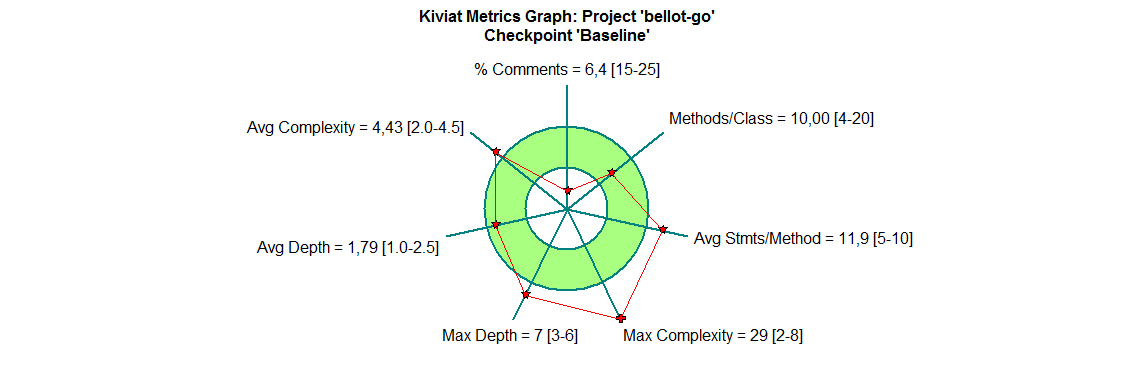
\includegraphics[width=\textwidth]{fig/bellot-go-20150105.png}
\end{center}
\end{frame}

\begin{frame}{SourceControl}
\begin{center}
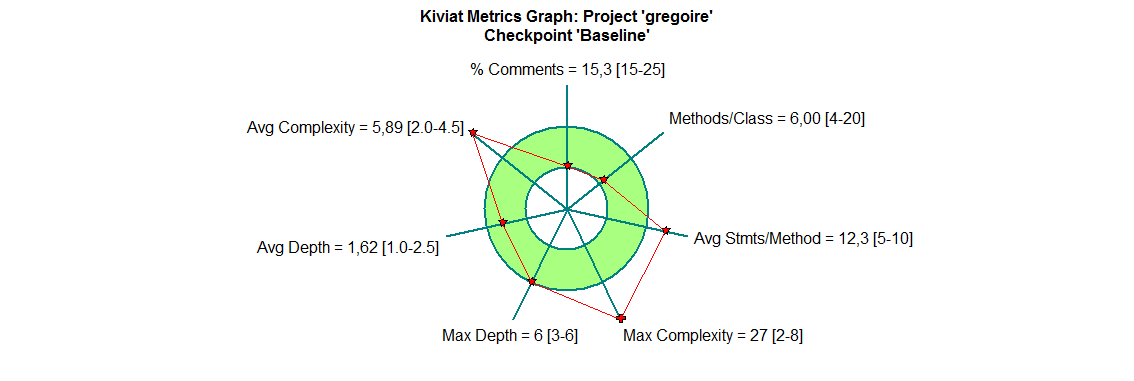
\includegraphics[width=\textwidth]{fig/gregoire-go-20150105.png}
\end{center}
\end{frame}

\begin{frame}{SourceControl}
\begin{center}
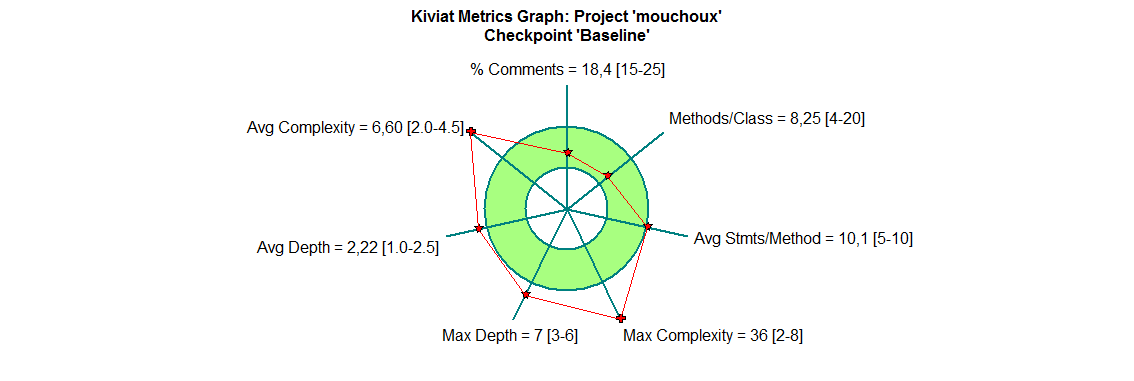
\includegraphics[width=\textwidth]{fig/mouchoux-go-20150105.png}
\end{center}
\end{frame}

\begin{frame}{SourceControl}
\begin{center}
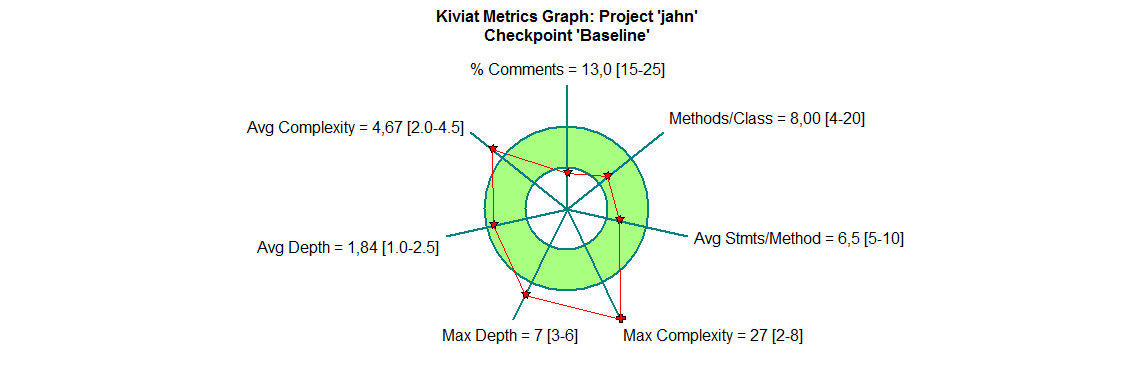
\includegraphics[width=\textwidth]{fig/jahn-go-20150105.png}
\end{center}
\end{frame}

\begin{frame}{SourceControl}
\begin{center}
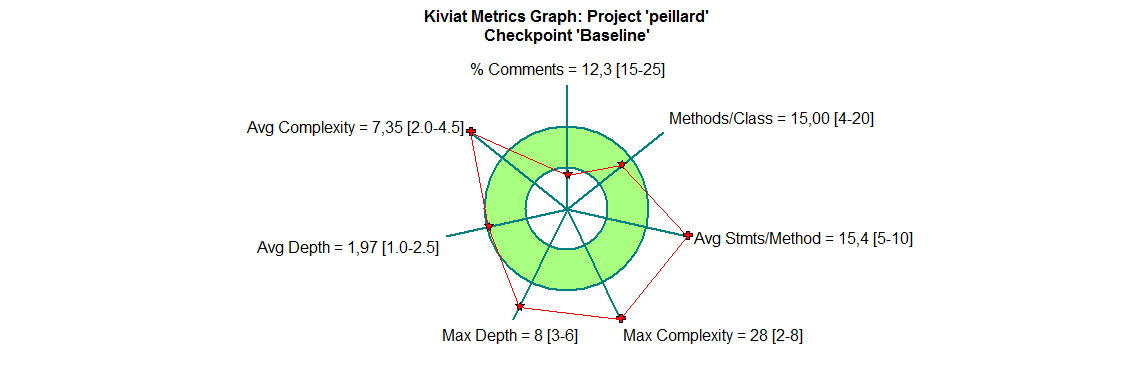
\includegraphics[width=\textwidth]{fig/peillard-go-20150105.png}
\end{center}
\end{frame}

\subsection{Cas particulier : couverture de code}

\begin{frame}{Couverture de code}
\begin{itemize}
\item Déterminer la couverture de tests n'est pas toujours très simple
\item Sans outils commerciaux... pas toujours compatibles avec autre chose que leurs propres outils de tests
\item Une méthode entièrement gratuite avec les outils GNU et Google Test
\begin{itemize}
\item des options de compilations appropriées dans \texttt{gcc}
\item \texttt{gcov} pour l'analyse de couverture
\item \texttt{lcov} pour le rendu
\end{itemize}

\end{itemize}
\end{frame}

\begin{frame}[fragile]
\begin{itemize}
\item Compilation du code 
\begin{verbatim}
g++ -I ../../../dev/local/gtest-1.7.0/include *.cpp 
	-L ../../../dev/local/gtest-1.7.0/ -lgtest 
	-o algogen_cov -p --coverage
\end{verbatim}
\item Exécution des tests
\begin{verbatim}
[~/tmp/algogen_cov/AlgoGen] moreau% ./algogen_cov 
[==========] Running 5 tests from 2 test cases.
...
[  PASSED  ] 5 tests.
\end{verbatim}
\item Analyse de couverture
\begin{verbatim}
gcov main.cpp
\end{verbatim}
\item Création d'un rendu (en HTML)
\begin{verbatim}
lcov -o user_test.info -c -f -d .
genhtml -o user_result user_test.info
\end{verbatim}
\end{itemize}
\end{frame}

\begin{frame}{Résultats (1/3)}
\begin{center}
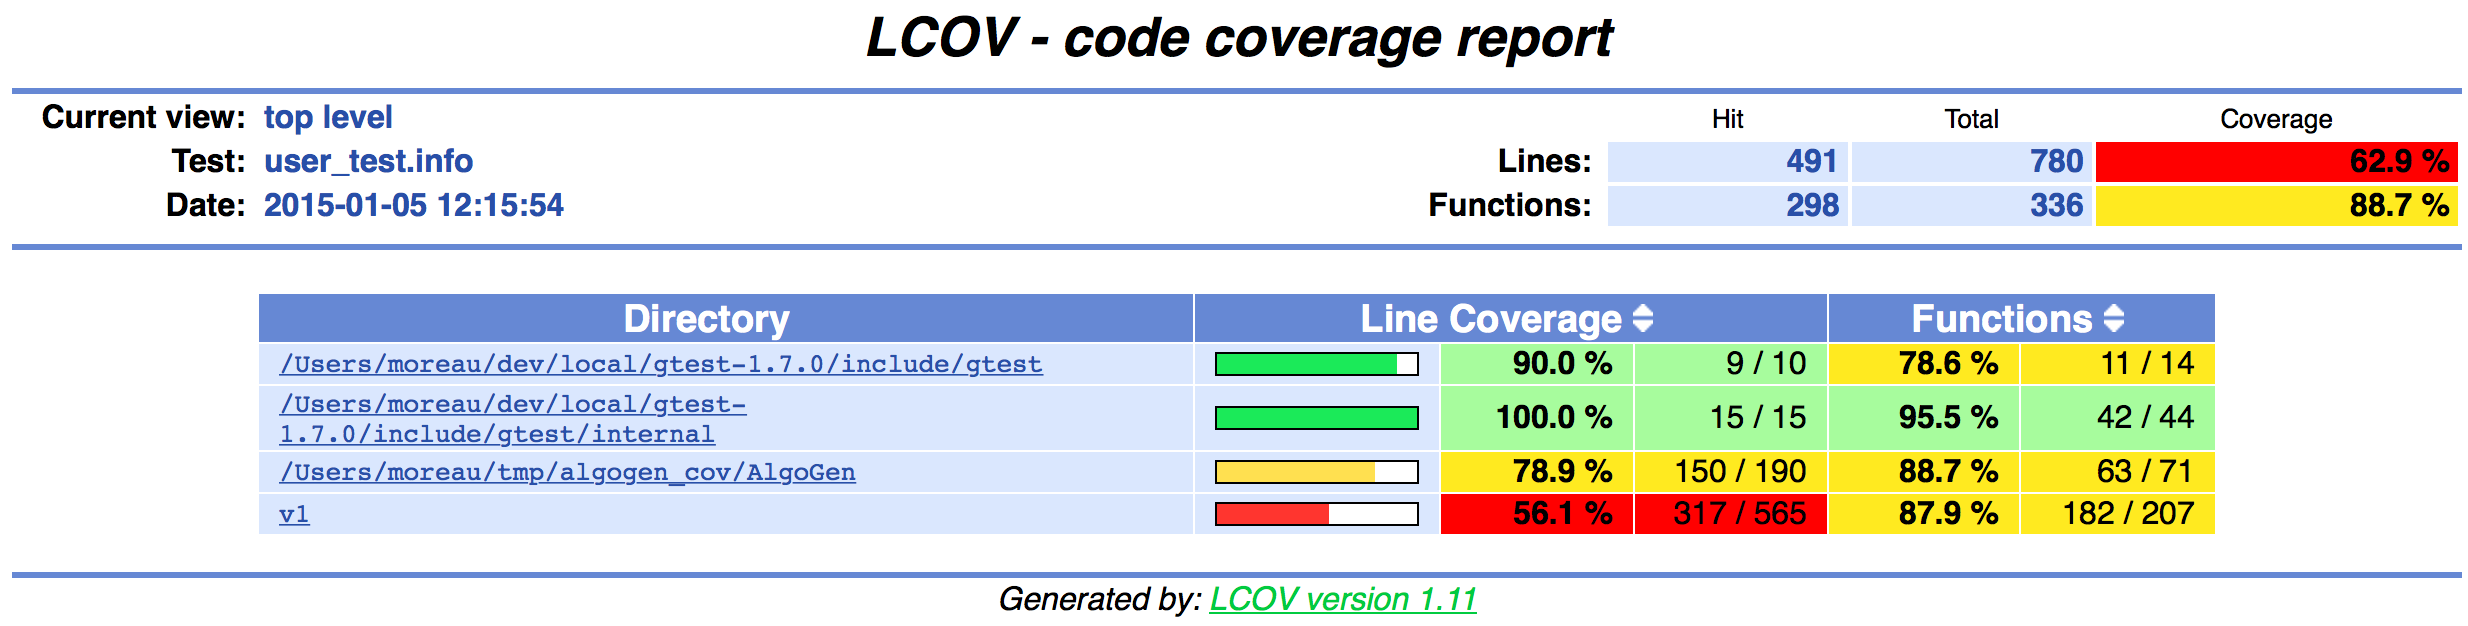
\includegraphics[width=.9\textwidth]{fig/lcov_top.png}
\end{center}
\begin{itemize}
\item Google Test a l'air plutôt bien testé...
\end{itemize}
\end{frame}

\begin{frame}{Résultats (2/3)}
\begin{center}
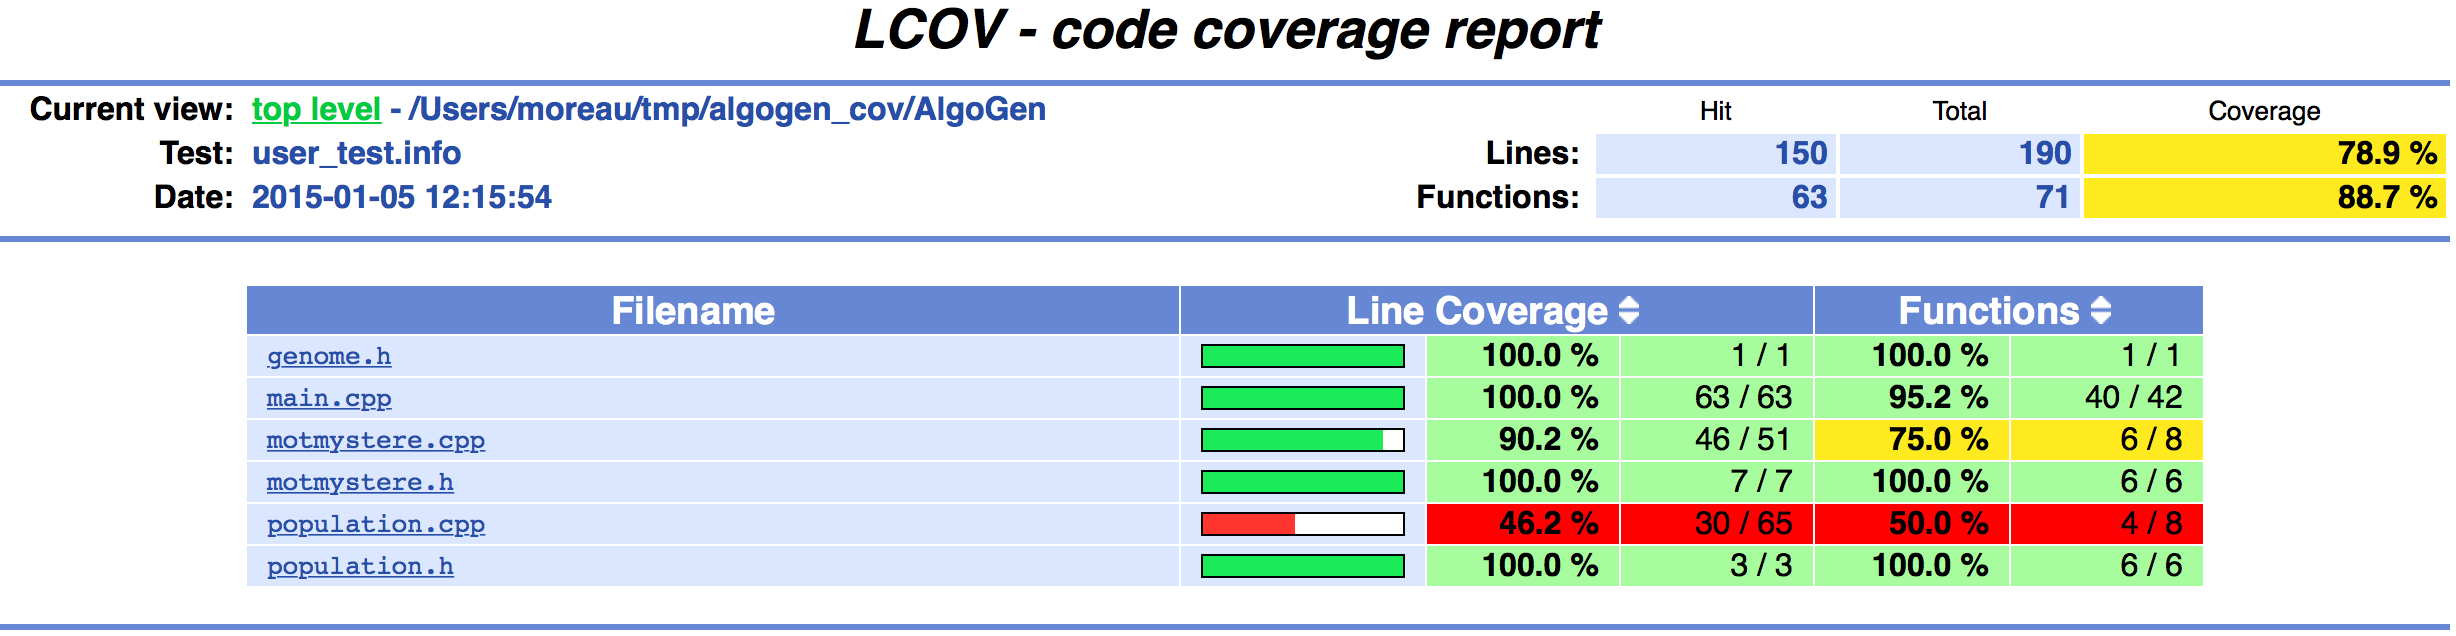
\includegraphics[width=.9\textwidth]{fig/lcov_algogen.png}
\end{center}
\begin{itemize}
\item Ca pourrait être pire !
\item Un problème avec la classe \textit{population} : plus difficile à tester compte tenu du traitement de listes.
\begin{itemize}
\item On peut aller plus dans le détail en cliquant sur chaque fichier
\end{itemize}
\end{itemize}
\end{frame}

\begin{frame}{Résultats (2/3)}
\begin{center}
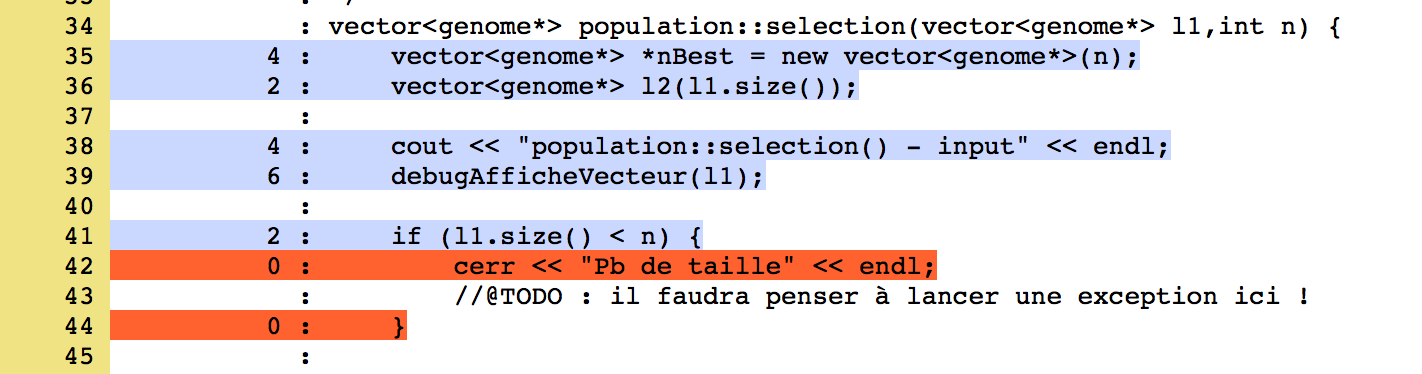
\includegraphics[width=.9\textwidth]{fig/lcov_untested.png}
\end{center}
\begin{itemize}
\item Exemple de cas pas testé
\item Le @todo était là avant...
\item Il y a bien pire après !
\end{itemize}
\end{frame}


\begin{frame}{Je ne suis pas tout seul...}
\begin{center}
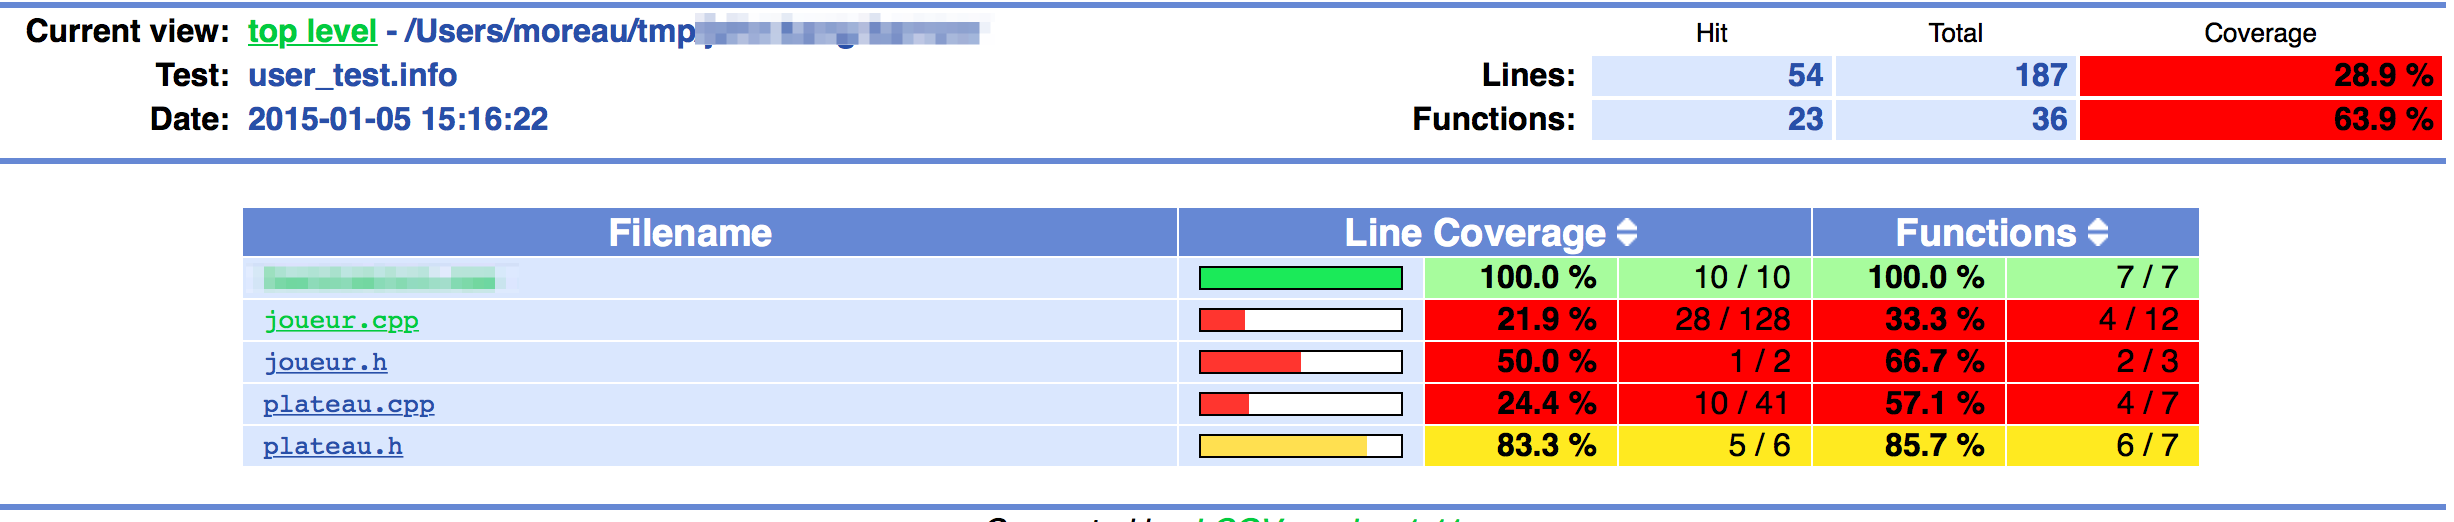
\includegraphics[width=.9\textwidth]{fig/lcov_tp.png}
\end{center}
\begin{itemize}
\item Exemple de jeu de Go (pris au hasard)
\end{itemize}
\end{frame}


\begin{frame}{A vous de jouer : programme du jour}
\begin{itemize}
\item Continuer le travail sur le jeu de Go et sur Github
\item Faire le point sur la qualité de son code
\begin{itemize}
\item avec SourceMonitor : \url{http://www.campwoodsw.com/sourcemonitor.html}
\item s'améliorer quand ça a du sens
\end{itemize}
\item Couverture de test
\begin{itemize}
\item Calculer sa couverture de test avec gcov/lcov
\item L'améliorer autant que possible
\end{itemize}
\item Documentation du programme
\begin{itemize}
\item Idée : utiliser les commentaires pour générer de la doc automatiquement
\item doxygen (\url{doxygen.org}) utilise les commentaires et quelques éléments de syntaxe spécifique pour générer des pages web (entre autres)
\end{itemize}
\end{itemize}
\end{frame}